% In the batch queue,  queue time becomes dominant but, at the same time, we
% have more freedom to decide the parameters of the slot.

\subsection{Experiments}

In this section we present experiments that aim to determine the performances of the NGE and to show how it provides a negligible overhead while introducing new functionalities.

Experiments consist in running AthenaMP instances by using NGE pilots where each AthenaMP simulates a pre-determined number of events taken from ATLAS workload.	
We present four groups of experiments in which we test the NGE for weak scalability, weak scalability with resubmission, strong scalability and heterogeous workloads.
For each group we vary the size of the pilots and the number of AthenaMP that are sent for execution. 
We collect data about the execution time of the pilots and the AthenaMP that are executed within them by considering all stages that these entities pass through during the execution.
Experiments have been performed out of production by using NGE's pilots on TITAN's batch queue. 
Because of TITAN's batch queue, the turnaround time of each run of our experiments is dominated by the time spent on TITAN's queue. Since we are interested only in the performances of the NGE, we do not provide data about queue time.

For the experiment, AthenaMP has been set to use all the 16 cores present on TITAN's nodes. 


\subsubsection{Weak scalability}

The experiment consists in running as many AthenaMP instances (also referred as tasks from now-on) as the number of nodes controlled by the pilot. Each AthenaMP have been assigned with 100 events whose simulation requires  ~$80$ minutes. 
 
Tasks do not experience queue within the pilot since there is one node for each ATLAS simulation. Therefore, delays are consequence of only three factors: i) the bootstrapping of the pilot on the nodes; ii) the manager that has to dispatch tasks to the pilot; iii) the time that the agent requires to spawn all of tasks on the nodes.

We tested different pilot sizes, i.e. : 250, 500, 1000 and 2000. For all of them the walltime was 2 hours.

Figure \ref{fig:weakScal1} depicts the average pilot duration, the average execution time of each tasks and the average time required to send a tasks for execution.  


\begin{figure}[!htb]
        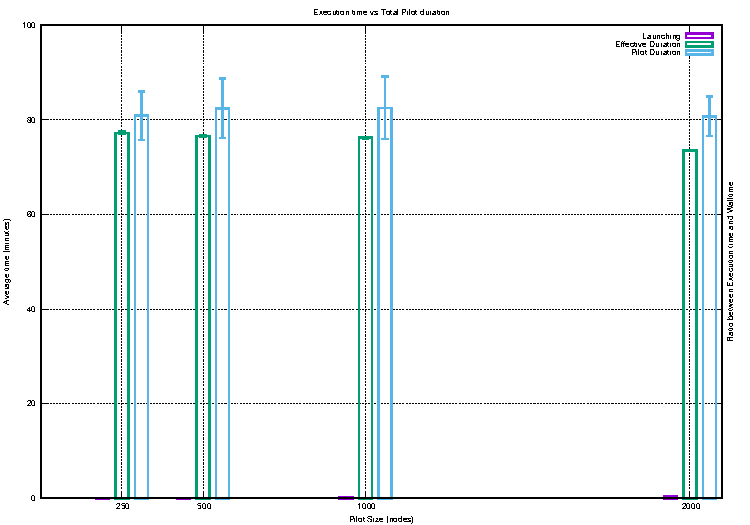
\includegraphics[width=0.5\textwidth]{./figures/NGE/Weak.pdf}
    \caption{Average pilot execution time, average tasks execution time and average launching time for pilot sizes: 250, 500, 1000 and 2000.}
\label{fig:weakScal1}
\end{figure}
\aanote{TO be commented as soon as the figure becomes definitive. Note that It would be better if we show the ratio between pilot duration and execution time}
\subsubsection{Weak scalability with resubmission }
This experiment is similar to the one presented above but in this case we want to test also the impact of submitting new simulations in place of those that end. Thus, we send to the pilot a number of tasks that is five times larger than the number of nodes. The reason behind this experiment is to stress the manager and the agent by pushing new tasks while others are ending their execution in such a way to increase the concurrency of these two components.

In order to perform the experiments in a reasonable amount of time, we reduced  the number of events that are simulated by Athena-MP to sixteen. This allows us to complete a task in ~25 minutes only. Note that the number of events has been chosen in such a way that all the cores of a node run one event.

We tested different pilot sizes, i.e. : 250, 500, 1000 and 2000. For all of them the walltime was 3 hours. 

Figure \ref{fig:weakScal2} \aanote{(DRAFT)}  depicts the average pilot duration, the average execution time of each tasks and the average time required to send a tasks for execution.  

\begin{figure}[!htb]
        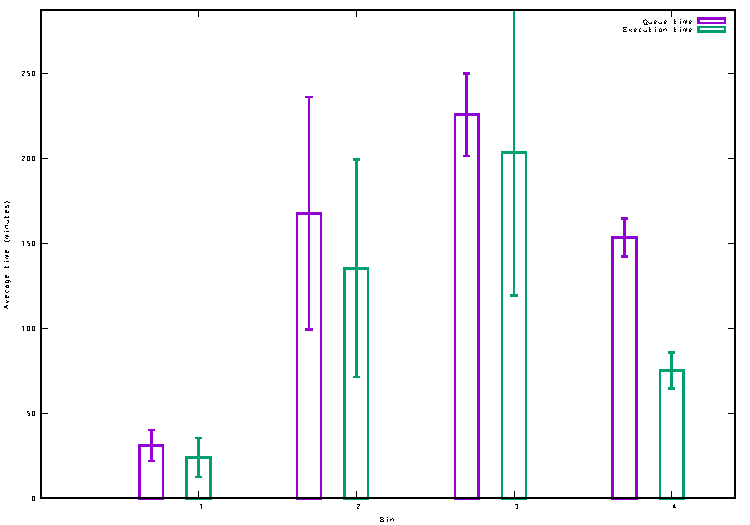
\includegraphics[width=0.48\textwidth]{./figures/draft/AvgT.pdf}
    \caption{Average pilot execution time, average tasks execution time and average launching time for pilot sizes: 250, 500, 1000 and 2000.}
\label{fig:weakScal2}
\end{figure}

\subsubsection{Strong scalability}

\subsubsection{Heterogeneous execution}






% For this reason, the second set of the experiments aims to find
%sub-optimal parameters with which we can minimize the trade-off between the size
%of a slot and the time spent in queue waiting for that slot to become available.
%In other words, we aim to minimize the completion time by finding the best
%trade-off between execution time and queue time.
%
%This execution model introduces slot utilization as one of the key factors for
%high-performances. This happens because, in order to minimize the time spent in
%queue, we might asks for slots in advance and, then we could not be able to
%saturate them when they become available. Thus, this strategy requires a new
%functionality that allows the job to receive and execute new events while it is
%already running on the resources. In order to do that we perform the experiments
%by using a new generation executor that implements such functionality.
%
%As last observation, it is important to point out that the percentage of
%utilization of a slot is minor problem with the current implementation because,
%due to the dynamics of the Backfill queue, PanDA has a high probability to
%re-acquire a slot immediately after it has released one\aanote{Are we able to
%quantify this ``immediately''?}.
